% Options for packages loaded elsewhere
% Options for packages loaded elsewhere
\PassOptionsToPackage{unicode}{hyperref}
\PassOptionsToPackage{hyphens}{url}
%
\documentclass[
  ignorenonframetext,
]{beamer}
\newif\ifbibliography
\usepackage{pgfpages}
\setbeamertemplate{caption}[numbered]
\setbeamertemplate{caption label separator}{: }
\setbeamercolor{caption name}{fg=normal text.fg}
\beamertemplatenavigationsymbolsempty
% remove section numbering
\setbeamertemplate{part page}{
  \centering
  \begin{beamercolorbox}[sep=16pt,center]{part title}
    \usebeamerfont{part title}\insertpart\par
  \end{beamercolorbox}
}
\setbeamertemplate{section page}{
  \centering
  \begin{beamercolorbox}[sep=12pt,center]{section title}
    \usebeamerfont{section title}\insertsection\par
  \end{beamercolorbox}
}
\setbeamertemplate{subsection page}{
  \centering
  \begin{beamercolorbox}[sep=8pt,center]{subsection title}
    \usebeamerfont{subsection title}\insertsubsection\par
  \end{beamercolorbox}
}
% Prevent slide breaks in the middle of a paragraph
\widowpenalties 1 10000
\raggedbottom
\AtBeginPart{
  \frame{\partpage}
}
\AtBeginSection{
  \ifbibliography
  \else
    \frame{\sectionpage}
  \fi
}
\AtBeginSubsection{
  \frame{\subsectionpage}
}
\usepackage{iftex}
\ifPDFTeX
  \usepackage[T1]{fontenc}
  \usepackage[utf8]{inputenc}
  \usepackage{textcomp} % provide euro and other symbols
\else % if luatex or xetex
  \usepackage{unicode-math} % this also loads fontspec
  \defaultfontfeatures{Scale=MatchLowercase}
  \defaultfontfeatures[\rmfamily]{Ligatures=TeX,Scale=1}
\fi
\usepackage{lmodern}

\ifPDFTeX\else
  % xetex/luatex font selection
\fi
% Use upquote if available, for straight quotes in verbatim environments
\IfFileExists{upquote.sty}{\usepackage{upquote}}{}
\IfFileExists{microtype.sty}{% use microtype if available
  \usepackage[]{microtype}
  \UseMicrotypeSet[protrusion]{basicmath} % disable protrusion for tt fonts
}{}
\makeatletter
\@ifundefined{KOMAClassName}{% if non-KOMA class
  \IfFileExists{parskip.sty}{%
    \usepackage{parskip}
  }{% else
    \setlength{\parindent}{0pt}
    \setlength{\parskip}{6pt plus 2pt minus 1pt}}
}{% if KOMA class
  \KOMAoptions{parskip=half}}
\makeatother


\usepackage{longtable,booktabs,array}
\usepackage{calc} % for calculating minipage widths
\usepackage{caption}
% Make caption package work with longtable
\makeatletter
\def\fnum@table{\tablename~\thetable}
\makeatother
\usepackage{graphicx}
\makeatletter
\newsavebox\pandoc@box
\newcommand*\pandocbounded[1]{% scales image to fit in text height/width
  \sbox\pandoc@box{#1}%
  \Gscale@div\@tempa{\textheight}{\dimexpr\ht\pandoc@box+\dp\pandoc@box\relax}%
  \Gscale@div\@tempb{\linewidth}{\wd\pandoc@box}%
  \ifdim\@tempb\p@<\@tempa\p@\let\@tempa\@tempb\fi% select the smaller of both
  \ifdim\@tempa\p@<\p@\scalebox{\@tempa}{\usebox\pandoc@box}%
  \else\usebox{\pandoc@box}%
  \fi%
}
% Set default figure placement to htbp
\def\fps@figure{htbp}
\makeatother





\setlength{\emergencystretch}{3em} % prevent overfull lines

\providecommand{\tightlist}{%
  \setlength{\itemsep}{0pt}\setlength{\parskip}{0pt}}



 


\makeatletter
\@ifpackageloaded{caption}{}{\usepackage{caption}}
\AtBeginDocument{%
\ifdefined\contentsname
  \renewcommand*\contentsname{Table of contents}
\else
  \newcommand\contentsname{Table of contents}
\fi
\ifdefined\listfigurename
  \renewcommand*\listfigurename{List of Figures}
\else
  \newcommand\listfigurename{List of Figures}
\fi
\ifdefined\listtablename
  \renewcommand*\listtablename{List of Tables}
\else
  \newcommand\listtablename{List of Tables}
\fi
\ifdefined\figurename
  \renewcommand*\figurename{Figure}
\else
  \newcommand\figurename{Figure}
\fi
\ifdefined\tablename
  \renewcommand*\tablename{Table}
\else
  \newcommand\tablename{Table}
\fi
}
\@ifpackageloaded{float}{}{\usepackage{float}}
\floatstyle{ruled}
\@ifundefined{c@chapter}{\newfloat{codelisting}{h}{lop}}{\newfloat{codelisting}{h}{lop}[chapter]}
\floatname{codelisting}{Listing}
\newcommand*\listoflistings{\listof{codelisting}{List of Listings}}
\makeatother
\makeatletter
\makeatother
\makeatletter
\@ifpackageloaded{caption}{}{\usepackage{caption}}
\@ifpackageloaded{subcaption}{}{\usepackage{subcaption}}
\makeatother

\usepackage{bookmark}
\IfFileExists{xurl.sty}{\usepackage{xurl}}{} % add URL line breaks if available
\urlstyle{same}
\hypersetup{
  pdftitle={Methods for Research and Policy Evaluation},
  pdfauthor={Paul Servais},
  hidelinks,
  pdfcreator={LaTeX via pandoc}}


\title{Methods for Research and Policy Evaluation}
\subtitle{Session 1}
\author{Paul Servais}
\date{}

\begin{document}
\frame{\titlepage}


\section{0. Introduction}\label{introduction}

\begin{frame}{Your instructor}
\phantomsection\label{your-instructor}
\begin{itemize}
\tightlist
\item
  Paul Servais,
  \href{mailto:paul.servais@sciencespo.fr}{\nolinkurl{paul.servais@sciencespo.fr}}.
\item
  Trained as physical engineer (Ecole Polytechnique de Bruxelles), then
  came to SciencesPo (Urban School), graduated last year
\item
  Now working on climate politics, comparative politics
\item
  I've been working on the electoral impacts of wind turbines on the
  vote for the RN
\end{itemize}
\end{frame}

\begin{frame}{Course objectives}
\phantomsection\label{course-objectives}
\begin{itemize}
\tightlist
\item
  Provide you with skills useful for:
\item
  Policy Evaluation
\item
  Quantitative research
\item
  With mathematical formalisation
\item
  Based on coding in R (on RStudio), with some Stata examples
\item
  Correlation is not causation !
\end{itemize}
\end{frame}

\begin{frame}{Course organisation}
\phantomsection\label{course-organisation}
\begin{itemize}
\tightlist
\item
  10' introduction
\item
  30' mathematical formalisation and coding examples
\item
  1h maths and coding exercices on R
\end{itemize}
\end{frame}

\begin{frame}{And you ?}
\phantomsection\label{and-you}
\begin{itemize}
\tightlist
\item
  Background ?
\item
  Objectives for the class ?
\end{itemize}
\end{frame}

\begin{frame}{Course material}
\phantomsection\label{course-material}
\begin{itemize}
\tightlist
\item
  Everything on
  \url{https://scpo-quantimethods.github.io/quantitative_methods_two/}
\item
  More structured than Moodle
\item
  Sessions, with clear codings outputs
\item
  Exercices
  \includegraphics[width=1\linewidth,height=\textheight,keepaspectratio]{images/image1.png}
\end{itemize}
\end{frame}

\begin{frame}{Course evaluation}
\phantomsection\label{course-evaluation}
\begin{itemize}
\tightlist
\item
  Simple pass/fail
\item
  Goal is to replicate or find a research question, by groups of two,
  and write a 5-pages document summarising the findings
\item
  The objective is clearly not to overload anybody with work, but to
  give useful tips and skills for the future !
\item
  Abstract
\item
  Intro - Theory - Methods - Results - Conclusion
\end{itemize}
\end{frame}

\begin{frame}{Sessions}
\phantomsection\label{sessions}
\begin{itemize}
\tightlist
\item
  \begin{enumerate}
  \tightlist
  \item
    Coding basics, and descriptive statistics
  \end{enumerate}
\item
  \begin{enumerate}
  \setcounter{enumi}{1}
  \tightlist
  \item
    Linear regressions
  \end{enumerate}
\item
  \begin{enumerate}
  \setcounter{enumi}{2}
  \tightlist
  \item
    Non-linear regressions
  \end{enumerate}
\item
  \begin{enumerate}
  \setcounter{enumi}{3}
  \tightlist
  \item
    Regression Discontinuity Design (RDD)\\
  \end{enumerate}
\item
  \begin{enumerate}
  \setcounter{enumi}{4}
  \tightlist
  \item
    Difference-in-differences (DiD) and panel data
  \end{enumerate}
\item
  \begin{enumerate}
  \setcounter{enumi}{5}
  \tightlist
  \item
    Instrumental Variables (IV)
  \end{enumerate}
\end{itemize}
\end{frame}

\begin{frame}{Other excellent sources}
\phantomsection\label{other-excellent-sources}
\begin{itemize}
\tightlist
\item
  Work by colleagues of my center (CEE) :
  \url{https://luissattelmayer.github.io/quant-2025/} ;
  \url{https://malo-jn.quarto.pub/introduction-to-r/} ;
  \url{https://www.rovny.org/methods-2-ed}
\item
  Work by other economists, who provide code examples and very detailed
  explanations : \textless\textgreater;
\end{itemize}
\end{frame}

\begin{frame}{Questions ?}
\phantomsection\label{questions}
\end{frame}

\section{Coding basics}\label{coding-basics}

\begin{frame}{Motivation}
\phantomsection\label{motivation}
\begin{itemize}
\tightlist
\item
  Our world is increasingly measured, monitored,
\item
  This creates loads of data about everything
\item
  The objectives of statistics is to find meaningful information in
  those data
\item
  Yet most of the time the data is imperfect, in terms of validity, and
  in terms of reliability
\end{itemize}
\end{frame}

\begin{frame}{Research problem and empirical evidence}
\phantomsection\label{research-problem-and-empirical-evidence}
\begin{itemize}
\tightlist
\item
  A research puzzle generally comes with identifying a puzzling
  relationship between two variables
\item
  Why Y despite X ? Because Z
\item
  Quantitative methods, and causal inference, are a way to assess the
  size of the effect of Z on Y and to measure its significance.
\end{itemize}
\end{frame}

\section{Descriptive statistics}\label{descriptive-statistics}

\begin{frame}{Descriptive statistics}
\phantomsection\label{descriptive-statistics-1}
\begin{itemize}
\tightlist
\item
  The first step in every statistical analysis
\item
  Describe the variables we work with

  \begin{itemize}
  \tightlist
  \item
    remove outliers, deal with missing values
  \item
    verify the quality of the data

    \begin{itemize}
    \tightlist
    \item
      range
    \item
      mean
    \item
      median
    \item
      standard deviation
    \end{itemize}
  \end{itemize}
\end{itemize}
\end{frame}

\begin{frame}{Random variables}
\phantomsection\label{random-variables}
\begin{itemize}
\tightlist
\item
  A variable with random outcomes, is called a random variable : eg. a
  census is generally built on a sample of individuals, randomly drawn
  from an overall population.
\item
  Categorical : finite amount of values/categories

  \begin{itemize}
  \tightlist
  \item
    Nominal : non-ordered eg. gender, the department where you live
  \item
    Ordinal : ranking of preferences eg. ranking your preferences from 1
    to 5
  \end{itemize}
\item
  Continuous/interval variables : infinite number of potential outcomes
  (in a given range)
\end{itemize}
\end{frame}

\begin{frame}{One dice example}
\phantomsection\label{one-dice-example}
\begin{itemize}
\tightlist
\item
  A typical example is the result of a six-faces dice, that you throw.
\item
  \(X\), the result of your dice, is a random variable
\item
  \(S_X = \{1,2,3,4,5,6\}\) is its set of potential outcomes
\item
  If your dice is not broken, \(P(X =1,2,3,4,5,6) = 1/6 = 0.1666667\).
\item
  The probability set is \(P_X = \{1/6, 1/6, 1/6, 1/6, 1/6, 1/6\}\).
  Each outcome comes with a probability.
\end{itemize}
\end{frame}

\begin{frame}[fragile]{One dice example - distribution}
\phantomsection\label{one-dice-example---distribution}
\begin{itemize}
\tightlist
\item
  You throw it a 1000 times. I randomly generate that variable in R,
  using \texttt{sample()}
\end{itemize}

\begin{verbatim}
[1] 2 4 1 6 5 4
\end{verbatim}

\begin{verbatim}
[1] 3.578
\end{verbatim}

\begin{verbatim}
[1] 2.950867
\end{verbatim}

\pandocbounded{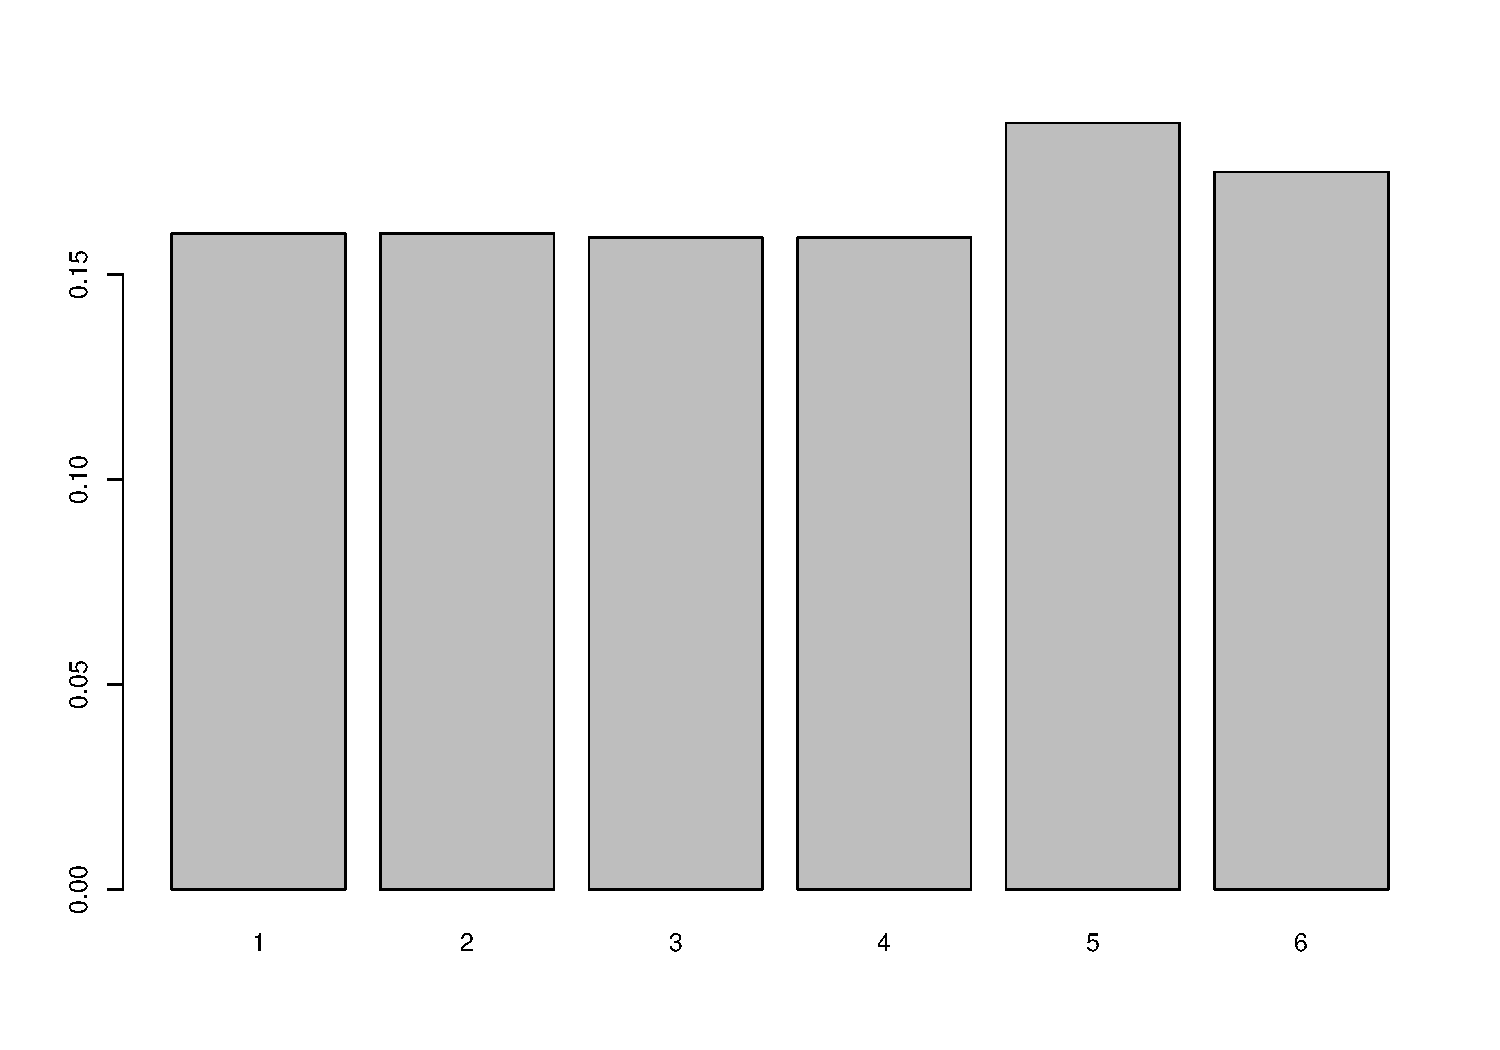
\includegraphics[keepaspectratio]{slides1_files/figure-beamer/unnamed-chunk-1-1.pdf}}
\end{frame}

\begin{frame}{Two dices example}
\phantomsection\label{two-dices-example}
\begin{itemize}
\tightlist
\item
  Now imagine that you have two dices
\item
  \(X_1\) is the result of dice 1, \(X_2\) is the result of dice 2
\item
  \(Y = X_1 + X_2\) is also a random variable;
\item
  If \(X_1\) and \(X_2\) are independent and can be distinguished
  (e.g.~different colors) \begin{equation}
  P(Y_{ij}) = P(X_1 = i)\times P(X_2 = j)
  \end{equation}
\item
  \(S = \{2,3,4,5,6,7,8,9,10,11,12\}\)
\item
  Yet here \(X_1\) and \(X_2\) are interchangeable\ldots{} Probabilities
  = ?
\end{itemize}
\end{frame}

\begin{frame}{Two dices example}
\phantomsection\label{two-dices-example-1}
\begin{array}{c|cccccc}
 & 1 & 2 & 3 & 4 & 5 & 6 \\
\hline
1 & \frac{1}{36} & \frac{1}{36} & \frac{1}{36} & \frac{1}{36} & \frac{1}{36} & \frac{1}{36} \\
2 & \frac{1}{36} & \frac{1}{36} & \frac{1}{36} & \frac{1}{36} & \frac{1}{36} & \frac{1}{36} \\
3 & \frac{1}{36} & \frac{1}{36} & \frac{1}{36} & \frac{1}{36} & \frac{1}{36} & \frac{1}{36} \\
4 & \frac{1}{36} & \frac{1}{36} & \frac{1}{36} & \frac{1}{36} & \frac{1}{36} & \frac{1}{36} \\
5 & \frac{1}{36} & \frac{1}{36} & \frac{1}{36} & \frac{1}{36} & \frac{1}{36} & \frac{1}{36} \\
6 & \frac{1}{36} & \frac{1}{36} & \frac{1}{36} & \frac{1}{36} & \frac{1}{36} & \frac{1}{36}
\end{array}
\end{frame}

\begin{frame}[fragile]{Distribution}
\phantomsection\label{distribution}
\begin{verbatim}
[1] 7 7 8 4 9 9
\end{verbatim}

\begin{verbatim}
[1] 7.0476
\end{verbatim}

\begin{verbatim}
[1] 2.442075
\end{verbatim}

\pandocbounded{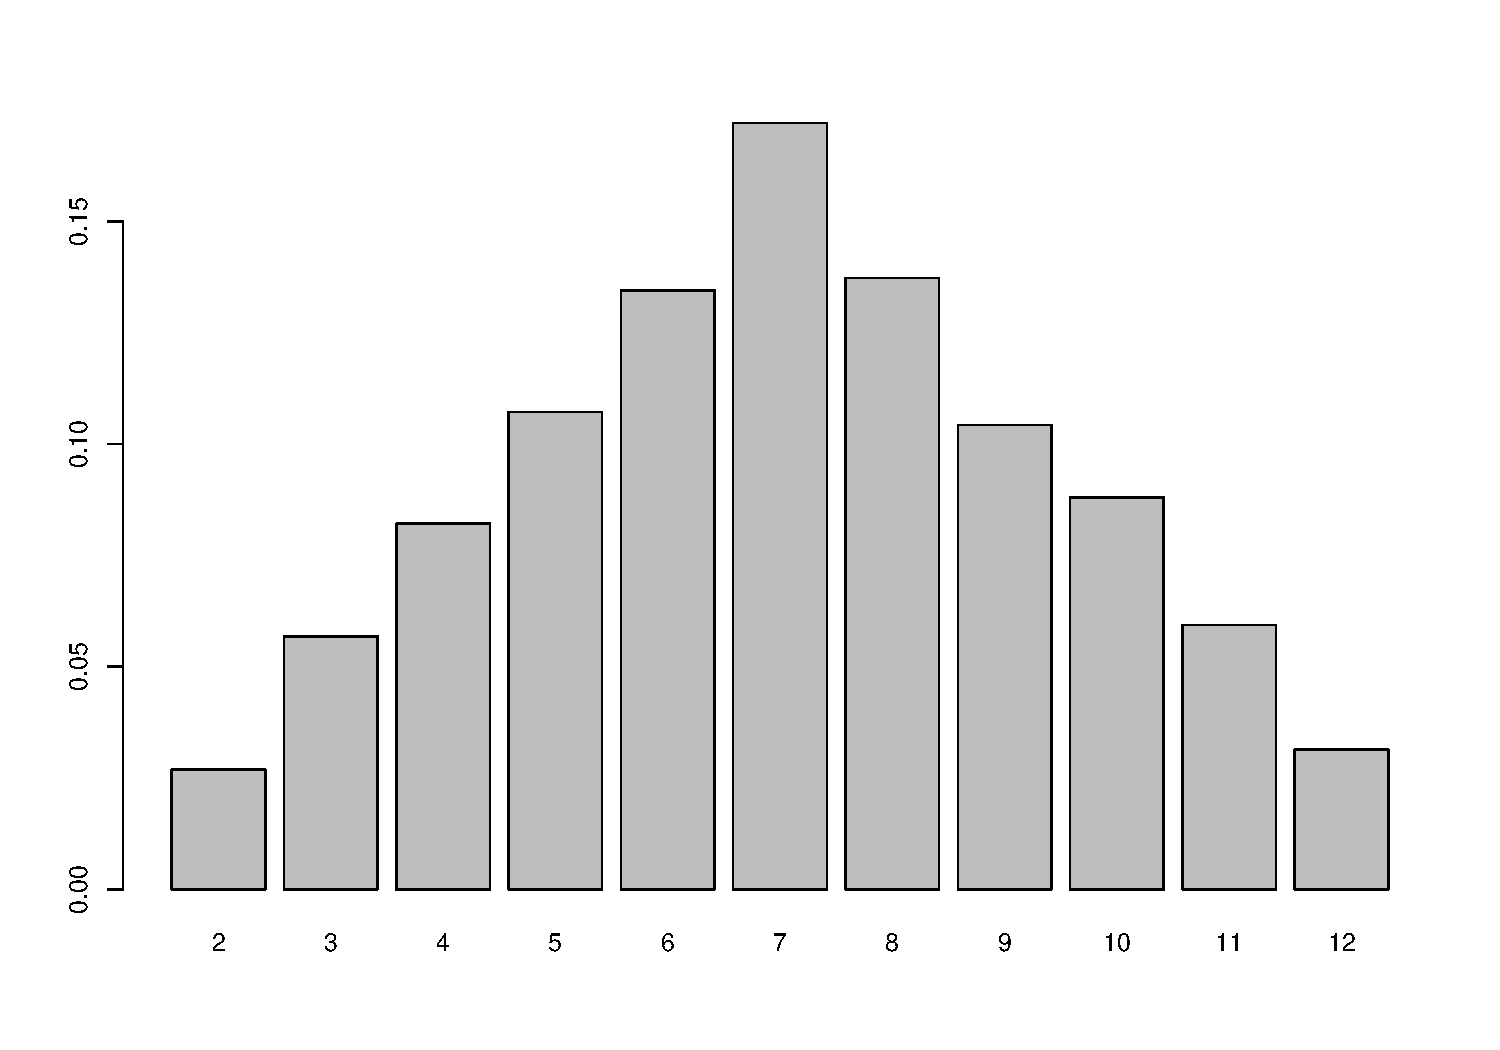
\includegraphics[keepaspectratio]{slides1_files/figure-beamer/unnamed-chunk-2-1.pdf}}
\end{frame}

\begin{frame}{Expectation and variance}
\phantomsection\label{expectation-and-variance}
\begin{itemize}
\tightlist
\item
  Imagine 7 is your \begin{equation}
  \text{E}(Y) = \sum_{i=1}^N Y_i * P(Y_i) = \bar{Y}
  \end{equation}
\item
  And you want to measure the dispersion around the mean called the
  variance : \begin{equation}
  \text{E}((Y_i-\bar{Y})^2) = \frac{1}{N} \sum_{i=1}^N (Y_i - \bar{Y})^2
  \end{equation}
\end{itemize}
\end{frame}

\begin{frame}{Conditional probability}
\phantomsection\label{conditional-probability}
\begin{itemize}
\tightlist
\item
  Now imagine that you know the value of one dice, but not the other.
\item
  Imagine \(X_1 =4\).
\item
  Set?
\item
  \(S_Y = \{5,6,7,8,9, 10\}\)
\item
  What are the probabilities ? \begin{equation}
  P(Y|X_1 = 4) = \frac{1}{6}
  \end{equation}
\item
  Hence, knowing \(X_1\) considerably influences the probabilities on Y!
\end{itemize}
\end{frame}

\begin{frame}{Conditional expectation}
\phantomsection\label{conditional-expectation}
\begin{itemize}
\tightlist
\item
  Knowing \(X_1 = 4\) therefore also changes the expectation :
  \begin{equation}
  \mathbb{E}(Y|X_1 = 4) = \frac{1}{6}(5+6+7+8+9+10) = 7.5
  \end{equation}
\end{itemize}

\pandocbounded{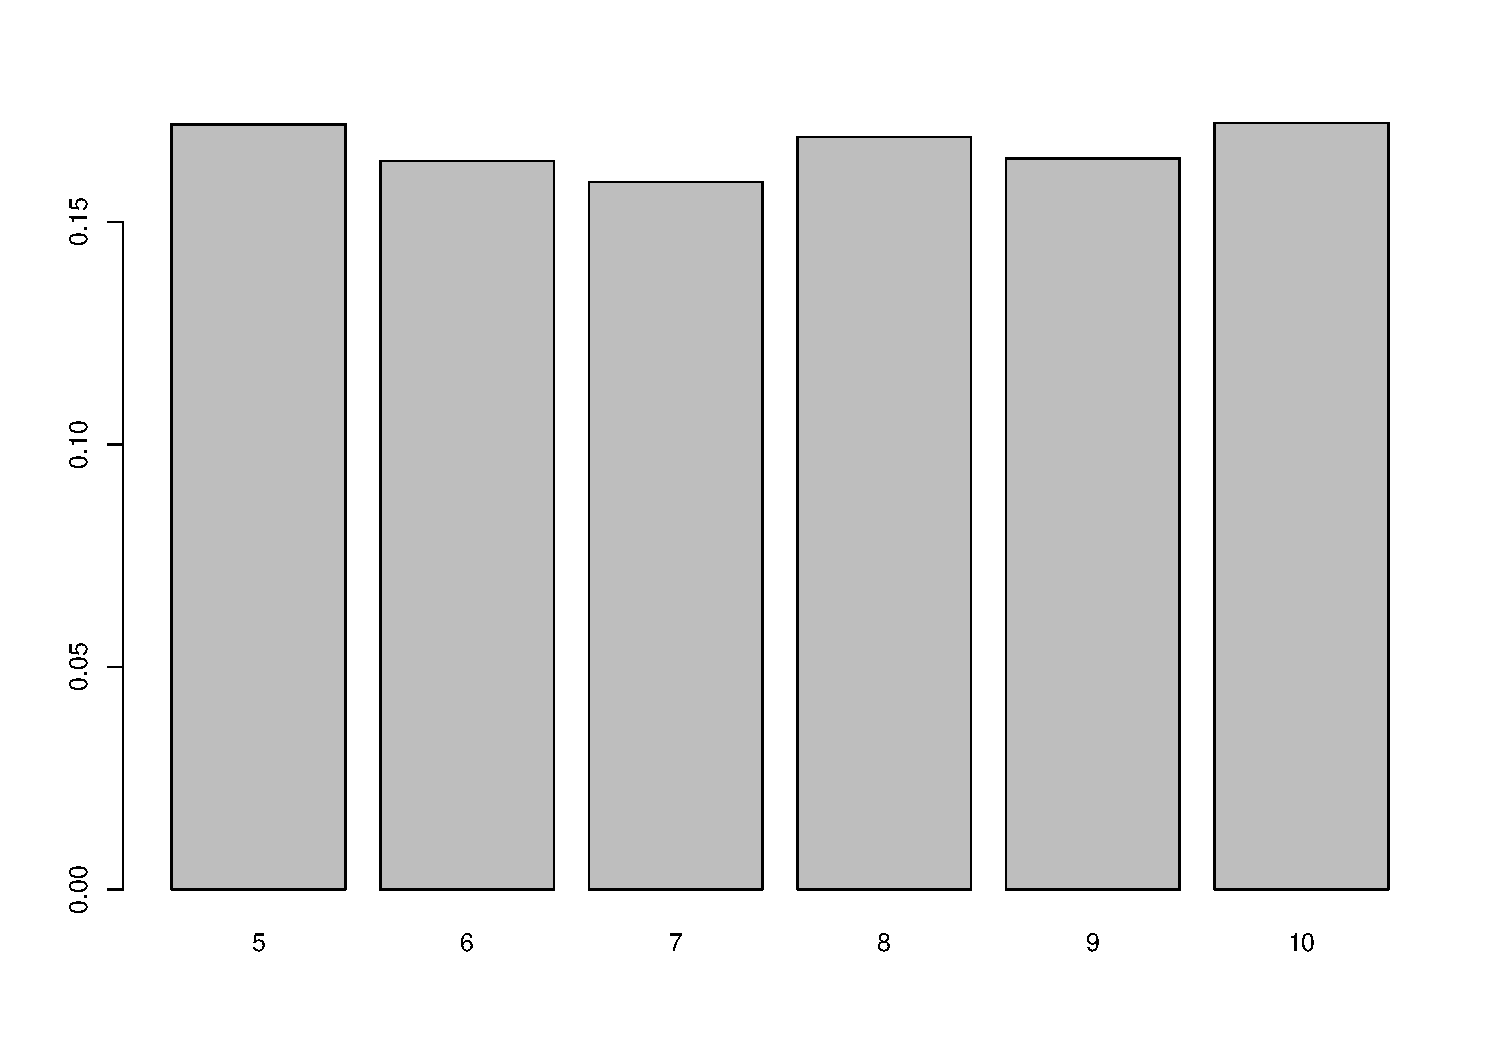
\includegraphics[keepaspectratio]{slides1_files/figure-beamer/unnamed-chunk-3-1.pdf}}
\end{frame}

\begin{frame}[fragile]{Towards continuity}
\phantomsection\label{towards-continuity}
\begin{itemize}
\tightlist
\item
  You have 1000 dices, with \(i = 1,2,3,..., 1000\) faces.
\item
  Values are all divided by \(i\).
\item
  You randomly pick 100 of these,
\item
  You throw each of them 10000 times
\item
  You report the sum as random variable Y
\end{itemize}

\begin{verbatim}
[1] 49.60694 44.62439 47.38863 52.88085 49.62886 47.82393
\end{verbatim}

\begin{itemize}
\tightlist
\item
  You now get closer to a continuous random variable\ldots{}
\item
  Your probability to obtain one specific value (eg. X = 43.503) becomes
  extremely small.
\end{itemize}
\end{frame}

\begin{frame}{Probability density for a continuous variable}
\phantomsection\label{probability-density-for-a-continuous-variable}
\pandocbounded{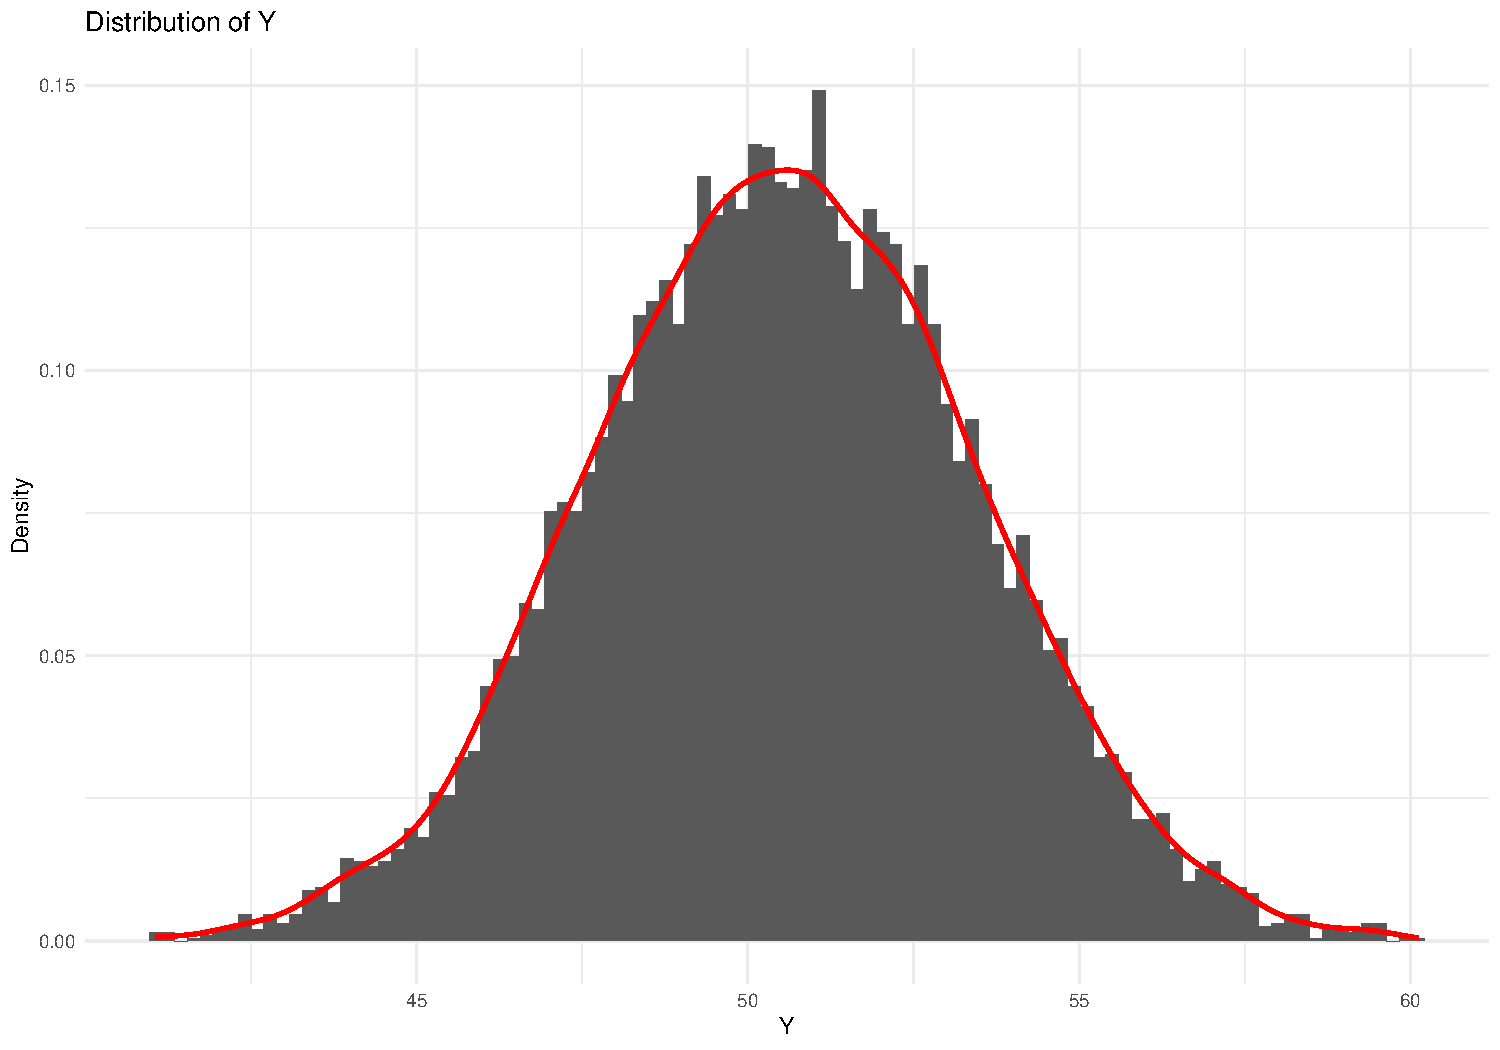
\includegraphics[keepaspectratio]{slides1_files/figure-beamer/unnamed-chunk-5-1.pdf}}
\end{frame}

\begin{frame}[fragile]{Real-life examples}
\phantomsection\label{real-life-examples}
\begin{itemize}
\tightlist
\item
  Imagine you work on the French communes
\item
  You seek to describe the median income in those communes
\item
  You only have access to a random sample of 10.000 of these
\end{itemize}

\pandocbounded{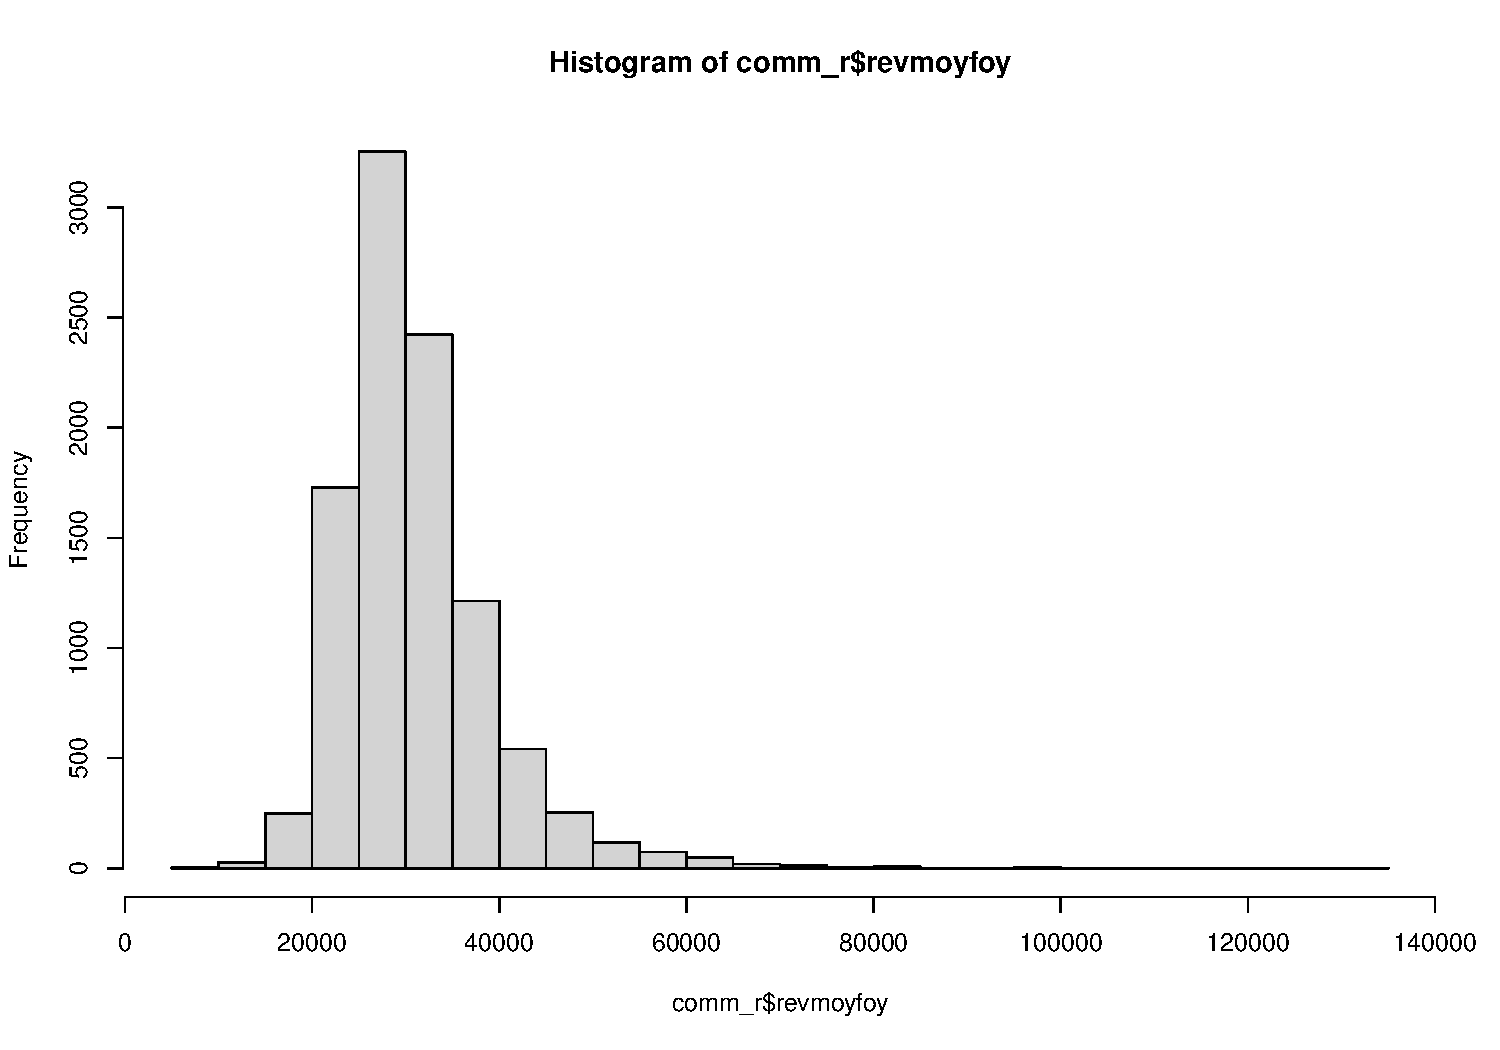
\includegraphics[keepaspectratio]{slides1_files/figure-beamer/unnamed-chunk-6-1.pdf}}

\begin{verbatim}
   Min. 1st Qu.  Median    Mean 3rd Qu.    Max.    NA's 
   8151   25816   29613   31106   34454  133022       9 
\end{verbatim}
\end{frame}

\begin{frame}[fragile]{Median income in those communes = ?}
\phantomsection\label{median-income-in-those-communes}
\begin{itemize}
\tightlist
\item
  Interval or categorical variable ?
\end{itemize}

\begin{verbatim}
[1] "numeric"
\end{verbatim}

\pandocbounded{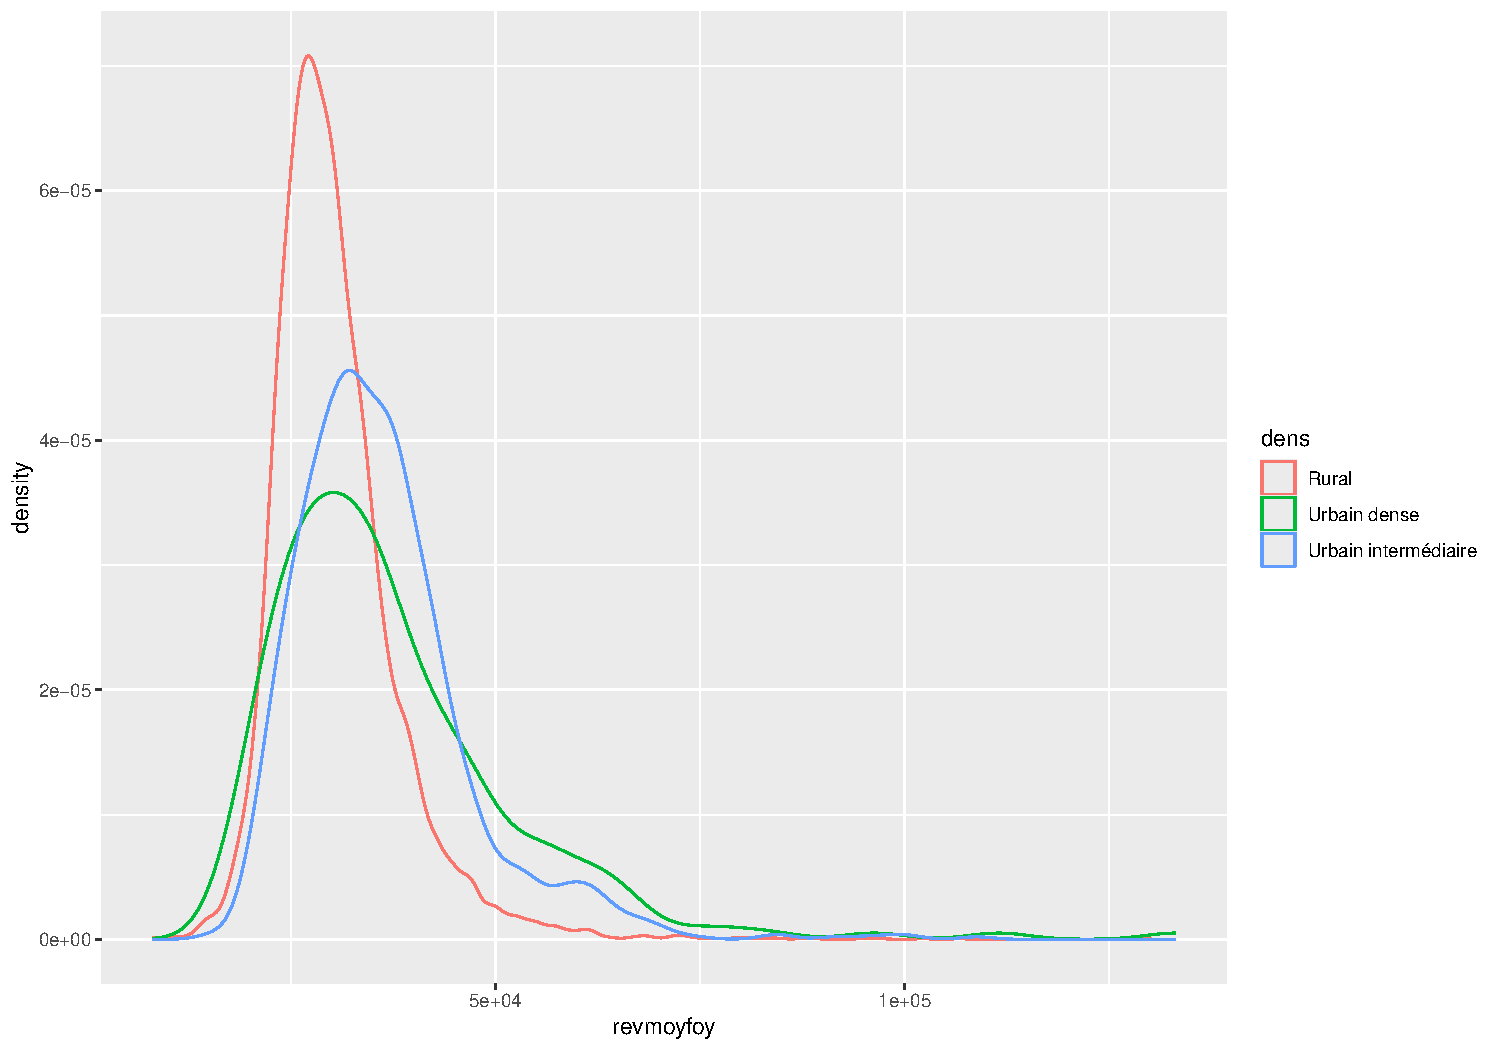
\includegraphics[keepaspectratio]{slides1_files/figure-beamer/unnamed-chunk-7-1.pdf}}
\end{frame}

\begin{frame}{S}
\phantomsection\label{s}
\end{frame}




\end{document}
